\documentclass[a4paper,oneside]{book}
\usepackage{anysize}
\usepackage{lastpage}
\usepackage{fancyhdr}
\usepackage{polyglossia}
\setdefaultlanguage[variant=uk]{english}
\usepackage{fontspec}
\usepackage{color}
\definecolor{bkg}{rgb}{0.9,0.9,0.9}
\definecolor{cmt}{rgb}{0.0,0.6,0.0}
\definecolor{boxbkg}{rgb}{0.9,0.95,1.0}
\usepackage{fancybox}
\usepackage{mdframed}
\usepackage{listings}
\defaultfontfeatures{Ligatures=TeX}
\usepackage{graphicx}
\graphicspath{{./logo/}{./img/}}
\usepackage[x11names]{xcolor}
\usepackage[colorlinks=true]{hyperref}
\usepackage{framed}
\usepackage{float}
\usepackage{wrapfig}
\restylefloat{figure}
\usepackage{makeidx}
\usepackage{listings}
\usepackage{amsmath}

\newtoggle{InString}{}% Keep track of if we are within a string
\togglefalse{InString}% Assume not initally in string

\lstset{
    backgroundcolor=\color{bkg},
    basicstyle=\small\ttfamily,
    breaklines=true,
    columns=fullflexible,
    numbers=left,
    numberstyle=\tiny,
    keywordstyle=\color{blue},
    commentstyle=\color{cmt},
    stepnumber=5,
    captionpos=b,
}
\lstdefinelanguage{json}{
    string=[s]{"}{"},
    showstringspaces=false,
    stringstyle=\color{purple},
    morecomment=[s][\color{black}\ttfamily]{\ \ \"}{\"},
    morecomment=[s][\color{purple}\ttfamily]{\ \ \ \ \ \"}{\"},
    keywords=[1]{true, false},
    keywordstyle=[1]\color{cyan},
    columns=flexible,
    keepspaces=true,
    morecomment=[l]{//},
}
\usepackage{caption}
\usepackage{subcaption}

\marginsize{1.5cm}{1.5cm}{0.5cm}{1.7cm}
\pagestyle{plain}
\setmainfont{Reporter}
\makeindex

\begin{document}
\begin{figure}[h]
  \includegraphics[width=\textwidth]{doc_head.jpg}
\end{figure}

\parindent=0pt
\parskip=0.25cm

\begin{center}
\fontsize{20}{21}\selectfont

\textbf{GazeToMouse}:\\
Usage of the \textbf{Tobii Eye Tracker 4C}\\
from within a \textbf{ztree} program\\
\vskip 6mm
Tutorial
\vskip 6mm

\fontsize{13}{14}\selectfont
Simon Maurer - \texttt{simon.maurer@humdek.unibe.ch}\\
\today
\end{center}

\tableofcontents

%==============================================================================
\chapter{Introduction}\label{sec.intro}
This documents describes how to use the \href{https://tobiigaming.com/eye-tracker-4c/}{Tobii Eye Tracker 4C} in order to track the gaze of a subject and feed the gaze data to the mouse device.
This allows to use the eye tracker to control the mouse pointer position such that the mouse pointer is placed at the screen coordinates where the subject is gazing at.
This documentation comes with a set of tools (executable .exe files) that provide this functionality as well as some auxiliary tools that help to calibrate and test the eye tracker.

The project aims at providing a set of executables which allow to use the \href{https://tobiigaming.com/eye-tracker-4c/}{Tobii Eye Tracker 4C} in conjunction with \href{http://www.ztree.uzh.ch/en.html}{ztree} to perform economic experiments.
The following set of executables are provided:
\begin{description}
    \item[TobiiCalibrate.exe] This program is a simple wrapper for the Tobii calibration tool.
        It launches the calibration GUI where the subject is led through the calibration process.
        The calibration data is stored in the current profile of the eye tracker engine.
    \item[TobiiGuestCalibrate.exe] This program is a simple wrapper for the Tobii guest calibration tool.
        Similar to \texttt{TobiiCalibrate.exe} it launches the calibration tool, however, the calibration data is stored in a guest profile.
    \item[TobiiTest.exe] This program is a simple wrapper for the Tobii eye tracking testing tool.
        It launches a GUI where the result of the calibration can be verified and a new calibration process can be started if required.
    \item[GazeToMouse.exe] This program uses the \href{http://developer.tobii.com/tobii-core-sdk/}{Tobii Core SDK} (default) or the \href{http://developer.tobii.com/tobii-pro-sdk/}{Tobii Pro SDK} to get the position on the screen where the subject is looking at.
        The mouse cursor position is updated to this position.
        As a consequence, the mouse cursor is controlled by the gaze of the subject.
        The gaze position on the screen (as well as pupil size or eye positions when using \href{http://developer.tobii.com/tobii-pro-sdk/}{Tobii Pro SDK}) are further logged to an output file.
        Instead of using an eye tracker device it is also possible to simply log the mouse coordinates.
        \texttt{GazeToMouse.exe} runs infinitely until it is terminated by an external command.
        This should \textbf{not} be done with a forced kill (e.g.~by executing the command \texttt{taskkill /F /IM GazeToMouse.exe} or by killing the task with the task manager) because it prevents the program from terminating gracefully.
        This as several consequences:
        \begin{itemize}
            \item open files are not closed properly and the data stream is cut off. This can lead to corrupt files.
            \item if the feature of hiding the mouse pointer is used, the mouse will remain hidden.
            \item memory is not freed properly.
        \end{itemize}
        Instead \texttt{taskkill /IM GazeToMouse.exe} should be used.
        This is done in the program \texttt{GazeToMouseClose.exe}.
    \item[GazeToMouseClose.exe] This program requests GazeToMouse.exe to close gracefully and logs these events to the log file.
    \item[ShowMouse.exe] This program allows to restore the standard mouse pointer.
        It might be useful if the program \texttt{GazeToMouse.exe} crashes or is closed forcefully such that the mouse pointer is not restored after terminating.
        The subject might end up with a hidden mouse pointer.
        A good solution for such a case is to install a shortcut to \texttt{ShowMouse.exe} on the desktop in order to execute it with the keyboard.
\end{description}


%==============================================================================
\chapter{Quick Start}
\label{sec.quick}
In order to get started with a quick experiment you need the following things (\emph{server} refers to the machine running \texttt{ztree} and \emph{client} refers to the machines running \texttt{zleaf}):
\begin{itemize}
    \item a \href{http://www.ztree.uzh.ch/en.html}{ztree} installation with a server and one or more clients.
        To install \texttt{ztree} download the latest \texttt{ztree} version from the \href{https://www.uzh.ch/ztree/ssl-dir/index.php}{download secetion}\footnote{https://www.uzh.ch/ztree/ssl-dir/index.php} (requires a license and a login, see Section~\ref{sec.ztree}) and extract the server file \texttt{ztree.exe} to the chosen installation path on the server and the client file \texttt{zleaf.exe} to the chosen installation path on each client.
        Throughout this documentation the installation paths of the \texttt{ztree} client and server will be referred to as \texttt{<zleaf path>} and \texttt{<ztree path>}, respectively.
    \item the \href{https://tobiigaming.com/getstarted/}{Tobii Eye Tracking Core Software} installed on each client.
        To install the software \href{https://tobiigaming.com/downloadlatest/?bundle=tobii-core}{download}\footnote{https://tobiigaming.com/downloadlatest/?bundle=tobii-core} and execute the installation file.
        The installation path of this software will be referred to as \texttt{<Tobii path>} throughout this documentation.
    \item the \href{https://tobiigaming.com/eye-tracker-4c/}{Tobii Eye Tracker 4C} mounted and connected on each client.
        When encountering connection problems follow \href{https://help.tobii.com/hc/en-us/articles/115000432589-Is-your-Eye-Tracker-4C-not-connecting-}{these}\footnote{https://help.tobii.com/hc/en-us/articles/115000432589-Is-your-Eye-Tracker-4C-not-connecting-} instructions which might help to solve the problem.
    \item the \href{http://phhum-g111-nns.unibe.ch:10012/TBI/TBI-tobii_eye_tracker_gaze}{GazeToMouse toolset} installed on each client.
        To install the toolset \href{http://phhum-g111-nns.unibe.ch:10012/TBI/TBI-tobii_eye_tracker_gaze/tree/master/release}{download}\footnote{http://phhum-g111-nns.unibe.ch:10012/TBI/TBI-tobii\_eye\_tracker\_gaze/tree/master/release} the latest version (requires a subscription, see Section~\ref{sec.gitlab}) and extract all files to an installation path of your choosing.
        The GazeToMouse installation path will be referred to as \texttt{<GazeToMouse path>} throughout this document.
    \item the ztree sample file.
        The file is located in \texttt{<GazeToMouse path>\textbackslash sample\textbackslash template.ztt}.
        Make sure to change the \texttt{Path} variable in \texttt{Background} of the sample file such that it points to \texttt{<GazeToMouse path>}.
\end{itemize}

The provided sample \texttt{ztree} program performs the following stages:
\begin{description}
    \item[Calibrate Eye Tracker]
        A guest calibration is performed where the Tobii calibration tool is started and the calibration data is stored in a guest profile within the Tobii eye tracker software.
        The calibration is very intuitive and has a game-like feel to it.
    \item[Test Eye Tracker]
        The Tobii eye tracker test tool is started which allows the subject or experimenter to verify the accuracy of the eye tracker.
        If the accuracy is not sufficient a recalibration can be started from within the test tool.
    \item[Gaze To Mouse]
        The gaze of the subject is tracked and transformed to mouse coordinates which allows to control the mouse pointer with the gaze of the subject.
    \item[Terminate]
        Terminates the gaze-to-mouse functionality and concludes this simple \texttt{ztree} program.
\end{description}

The behaviour of the GazeToMouse toolset can be configured with a configuration file (see Chapter~\ref{sec.config} for more details).
A sample configuration file is provided in \texttt{<GazeToMouse path>\textbackslash sample\textbackslash config.json} that can be modified to suit different requirements.
Copy the configuration file either to \texttt{<GazeToMouse path>} or \texttt{<zleaf path>} and modify it there.

%------------------------------------------------------------------------------
\section{Requesting Access to the Latest \texttt{ztree} Release}
\label{sec.ztree}
To download the latest release of the \texttt{ztree} software a login must be requested \href{https://www.uzh.ch/ztree/ssl-dir/index.php?action=obtain}{here}\footnote{https://www.uzh.ch/ztree/ssl-dir/index.php?action=obtain}.
Make a careful note of the terms and conditions.

%------------------------------------------------------------------------------
\section{Requesting a TPF GitLab Account}
\label{sec.gitlab}
The necessary code for what is described in this document is contained in a \texttt{GitLab} instance running on the \href{http://phhum-g111-nns.unibe.ch:10012/}{TPF server}\footnote{http://phhum-g111-nns.unibe.ch:10012/}.

Please send a mail to \href{tpf@humdek.unibe.ch}{TPF}\footnote{tpf@humdek.unibe.ch} with a request, specifying your name, the name of the TPF project you are interested in (e.g~\texttt{GazeToMouse}) and a user name which you would like to have on \texttt{GitLab}.


%==============================================================================
\chapter{Use GazeToMouse Toolset in Ztree}
\label{sec.gazetomouse}
This chapter provides instructions of how to use the Tobii Eye Tracker 4C in a \texttt{ztree} program.
In order to do this there are two main points to understand:
\begin{enumerate}
    \item How does the Tobii Eye Tracker 4C work
    \item How to execute 3rd party applications from within \texttt{ztree}
\end{enumerate}
The first point is addressed in Section~\ref{sec.eyetracker} and the second point in Section~\ref{sec.external}.

%------------------------------------------------------------------------------
\section{Basic Principles of the Tobii Eye Tracker 4C}
\label{sec.eyetracker}
The eye tracker is mounted on the bottom of the screen such that its cameras are able to capture the eyes of the subject.
Several infrared LEDs are visible once the device is connected and properly working (see Figure~\ref{fig.eyetracker}).
This requires the Tobii software to be installed and running.
\begin{figure}[ht]
    \centering
    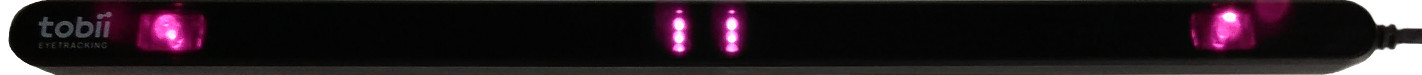
\includegraphics[width=0.95\textwidth]{eye_tracker.jpg}
    \caption{Picture of the Tobii Eye Tracker 4C in operation.}
    \label{fig.eyetracker}
\end{figure}

In order for the eye tracker to being able to track the gaze of the subject it must be calibrated.
A user-friendly calibration tool is included in the Tobii software package.
For each person different calibration data must be stored.
For this reason the Tobii software supports multiple user profiles which can be switched on the fly.
Given that in an economic experiment a workstation is used by a subject only once it is suggested to use the \emph{Guest} profile to store the eye tracker calibration data.
The guest calibration can be launched by executing the \texttt{TobiiGuestCalibrate.exe} program, provided in the toolset.
Once the eye tracker is calibrated for a subject, everything is ready.

%------------------------------------------------------------------------------
\section{Execute 3rd Party Applications in \texttt{ztree}}
\label{sec.external}
In a first step, it is useful to define a global variable \texttt{Path} in a \texttt{ztree} program that points to the location of the toolset.

In order to define a path
\begin{enumerate}
    \item click on the last table in \texttt{Background}
    \item choose the menu \texttt{Treatment} $\rightarrow$ \texttt{New Program...}
    \item define the path of the installation folder of the \texttt{GazeToMouse} toolset, i.e.~\texttt{<GazeToMouse path>} as \texttt{Path} variable\\
        (e.g.~\texttt{Path="C:\textbackslash\textbackslash Users\textbackslash\textbackslash Max Muster\textbackslash\textbackslash Documents\textbackslash\textbackslash My Experiment\textbackslash\textbackslash GazeToMouse\textbackslash\textbackslash";}). \\
        Note that two backslashes are required for each path delimiter because in ztree \texttt{\textbackslash} is used as escape character.
\end{enumerate}

When writing the different stages of a \texttt{ztree} program, calls to external applications can be made.
This can be achieved as follows:
\begin{enumerate}
    \item click on the position in your \texttt{ztree} experiment file where you want to include the call to the external program
    \item choose the menu \texttt{Treatment} $\rightarrow$ \texttt{New External Program...}
    \item choose \texttt{Run on z-Leaf}
    \item add the call to the external program to the field \texttt{Command Line} \\
        (e.g~a call to the guest calibration tool: \texttt{<><Path|-1>TobiiGuestCalibrate.exe}\\
        Note that the \texttt{Path} variable is used to indicate the location of the program.
        Figure~\ref{fig.extcall} shows an example of calling the Tobii guest calibration tool.
\end{enumerate}
\begin{figure}[ht]
    \centering
    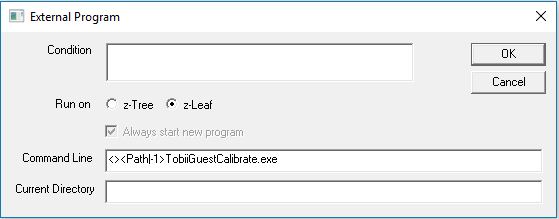
\includegraphics[width=0.6\textwidth]{ztree_extcall.png}
    \caption{External program call definition in \texttt{ztree}. The variable \texttt{Path} must be globally defined.}
    \label{fig.extcall}
\end{figure}

%==============================================================================
\chapter{Configuration of the \texttt{GazeToMouse} Toolset}
\label{sec.config}
The \texttt{GazeToMouse} toolset can be configured to work with different installations.
It allows to specify installation paths and gives some control over implemented features (e.g.~mouse hiding, gaze filtering, or data logging).
The Listing~\ref{lst.config} shows the default configuration values and provides an explanation for each value.
The configuration file contains detailed descriptions for each parameter.
It is recommended to go through all the configuration parameters and read the description in order to get an understanding of the available configuration options.

\lstinputlisting[language=json, caption={Default configuartion values},label=lst.config]{../sample/config.json}

Note that the configuration file follows the \texttt{json} syntax which must not be violated.
If the following points are respected, no problem should arise:
\begin{itemize}
    \item the configuration parameters are enclosed in `\texttt{\{}' and `\texttt{\}}'.
    \item all configuration parameters are of the form \texttt{"key":value} where \texttt{"key"} must not be changed.
    \item each configuration line ends with a `\texttt{,}' except for the last line where it is omitted.
    \item the Windows path delimiter `\texttt{\textbackslash}' must be escaped (i.e.~ write `\texttt{\textbackslash\textbackslash}' when describing a path)
    \item \texttt{json} supports standard data types (e.g. integer, boolean, string).
        Use the same type as the default value.
    \item everything following a `\texttt{//}' is considered a comment.
\end{itemize}

Each executable of the toolset uses the same common configuration file.
The configuration file must be named \texttt{config.json} and is read from the following places with the indicated priority:
\begin{enumerate}
    \item in the directory of the caller, i.e~in \texttt{<zleaf path>}
    \item in the directory of the executables, i.e.~in \texttt{<GazeToMouse path>}
\end{enumerate}
If no configuration file can be found, the default values are used.

\begin{mdframed}[backgroundcolor=boxbkg]\textbf{\color{red}Warning:}
    A word of warning when using the mouse hiding feature.
    This feature hides the mouse when running \texttt{GazeToMouse.exe}.
    If \texttt{GazeToMouse.exe} is forcefully closed or crashes, the mouse pointer stays hidden.
    For such cases the \texttt{ShowMouse.exe} utility can be used to restore the mouse pointer.
\end{mdframed}

%------------------------------------------------------------------------------
\section{Output File}
When running the program \texttt{gazeToMouse.exe} an output file can be generated which holds the gaze data provided by the Tobii engine.
The output file is saved in the directory specified by \texttt{OutputPath} in \texttt{config.json}.
The name of the output file follows the form
\begin{lstlisting}
<yyyyMMddTHHmmss>_<hostName>_<ConfigName>_gaze[_err-<code>].txt
\end{lstlisting}
where
\begin{itemize}
    \item \texttt{<yyyyMMddTHHmmss>} is replaced by the timestamp indicating when the file was created (e.g. 20180129T085521 stands for 29.01.2018 08:55:21).
    \item \texttt{<hostName>} is replaced by the name of the machine
    \item \texttt{<ConfigName>} is replaced by the configuration value \texttt{"ConfigName"} as specified in the configuration file (see Listing~\ref{lst.config} for more details)
    \item \texttt{[\_err-<code>]} is either omitted if no error occurred during the experiment or indicates data errors where
        \begin{itemize}
            \item \texttt{<code>} is replaced by an error code which is a binary string where each character can either be 1, indicating an error or 0, indicating no error (see Section~\ref{sect.data.error})
        \end{itemize}
\end{itemize}

An output file is only generated if the parameter \texttt{"DataLogWriteOutput"} in the configuration file is set to \texttt{true} (which is the default).
The presentation of the gaze data is configurable with the help of the parameters \texttt{"DataLogColumnOrder"}, \texttt{"DataLogColumnTitle"}, \texttt{"DataLogFormatDiameter"}, \texttt{"DataLogFormatOrigin"}, and \texttt{"DataLogFormatTimeStamp"} (see Listing~\ref{lst.config} for more details).

By default the \href{http://developer.tobii.com/tobii-core-sdk/}{Tobii Core SDK} is used (parameter \texttt{"TobiiSDK"} is set to 0) and only the timestamps and the x and the y coordinates of the gaze points are available.
A gaze point describes a point on the screen in x and y coordinates (pixel values) the user is gazing at.
This coordinate system is called \emph{Active Display Coordinate System (ADCS)} and is illustrated in Figure~\ref{fig.adcs}.
\begin{figure}[ht]
    \centering
    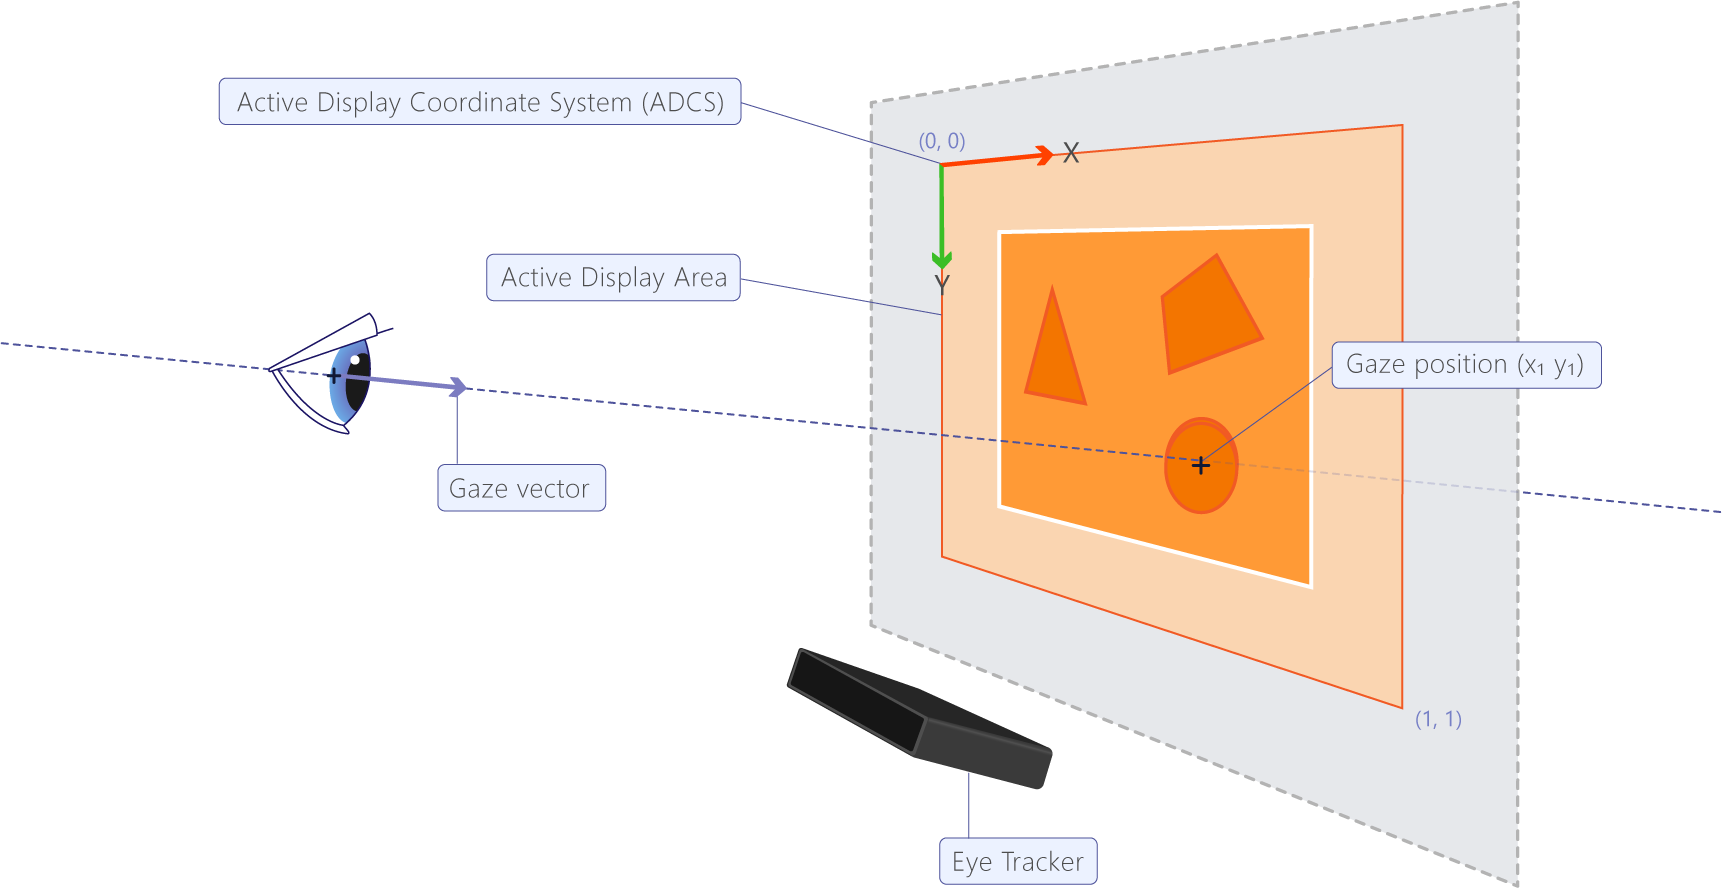
\includegraphics[width=0.8\textwidth]{adcs.png}
    \caption{The Active Display Coordinate System (ADCS). Figure source: \href{http://developer.tobiipro.com/commonconcepts/coordinatesystems.html}{Tobii}}
    \label{fig.adcs}
\end{figure}

By default, the system is configured to log the timestamp of when the gaze point was captured by the eye tracker (data field number 0) and the x and y coordinates of the gaze point (data field numbers 1 and 4, respectively).
Hence, the parameter \texttt{"DataLogColumnOrder"} is set to the value \texttt{"\{0\}\textbackslash t\{1\}\textbackslash t\{4\}"} in order to not bloat the output file with unnecessary header data.
This produces an output file that is similar to the following:
\lstset{columns=flexible}
\lstset{keepspaces=true}
\begin{lstlisting}
Timestamp   coord-x coord-y
12:51:55.409    426 342
12:51:55.420    430 341
12:51:55.431    431 341
...
\end{lstlisting}

When opening the file with a spreadsheet software such as LibreOffice Calc or Microsoft Office Excel two things need to be considered:
\begin{enumerate}
    \item The column delimiter needs to be set to the delimiter set in the configuration file (\texttt{'\textbackslash t'} by default).
    \item The language needs to be set to the language of the windows system where the configuration file was produced.
        This is important because numbers are represented differently in different languages and depending on the settings, commas might be interpreted as delimiters when they are not.
\end{enumerate}

When using \href{http://developer.tobii.com/tobii-pro-sdk/}{Tobii Pro SDK}, much more values are provided and can be logged to the output file.
This includes the pupil diameters of each eye as well as the eye positions in space.
The latter uses a coordinate system which is called \emph{User Coordinate System (UCS)}.
The UCS is illustrated in Figure~\ref{fig.ucs}.
\begin{figure}[ht]
    \centering
    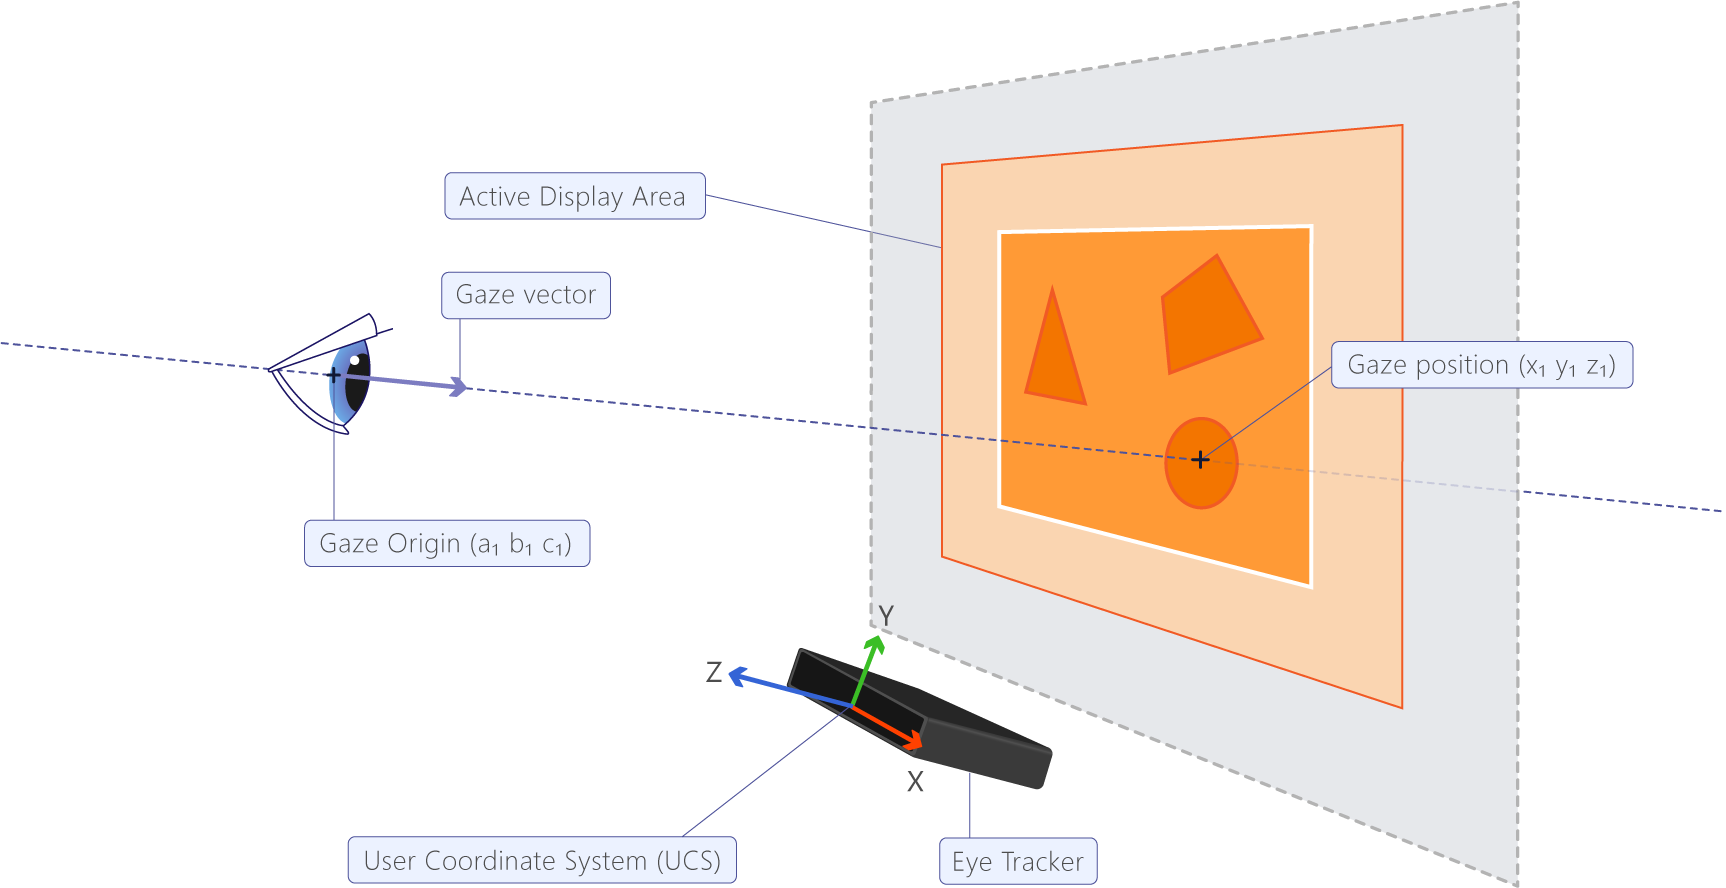
\includegraphics[width=0.8\textwidth]{ucs.png}
    \caption{The User Coordinate System (UCS). Figure source: \href{http://developer.tobiipro.com/commonconcepts/coordinatesystems.html}{Tobii}}
    \label{fig.ucs}
\end{figure}

In order to log additional data fields, the parameter \texttt{"DataLogColumnOrder"} must be modified by adding the required numbers, representing different data fields.
For example, to log all raw data fields (omitting any data field that is computed from raw data) the following string can be used:
\begin{lstlisting}
"DataLogColumnOrder": "{0}\t{2}\t{3}\t{5}\t{6}\t{7}\t{8}\t{10}\t{11}\t{12}\t{13}\t{14}\t{15}\t{16}\t{17}\t{18}\t{19}\t{23}\t{24}"
\end{lstlisting}

When using the empty string, all possible data fields are logged:
\begin{lstlisting}
"DataLogColumnOrder": ""
\end{lstlisting}

\subsection{Data Fields}
The comments above the parameter \texttt{"DataLogColumnOrder"} in the configuration file (see Listing~\ref{lst.config}) provide a short description for each available data field.
In the following some further information is provided.

The following five data field types with individual data fields are provided:
\begin{enumerate}
    \item timestamps indicating when the data was sampled by the eye tracker (field number: 0)
    \item gaze point ADCS coordinates (see Figure~\ref{fig.adcs}) as pixel values
        \begin{description}
            \item[Mouse Tracker] \hfill
                \begin{itemize}
                    \item the x and y coordinates of the mouse pointer\\
                        (field numbers: 1 and 4)
                \end{itemize}
            \item[Tobii Core SDK] \hfill
                \begin{itemize}
                    \item the average x and y coordinates where filtering depends on parameter "GazeFilterCore"\\
                        (field numbers: 1 and 4)
                \end{itemize}
            \item[Tobii Pro SDK] \hfill
                \begin{itemize}
                    \item raw x and y coordinates of the left and the right eye\\
                        (field numbers: 2, 3, 5, and 6)
                    \item the average x and y coordinates which are computed from raw data as defined by Equation~\ref{eq.average}\\
                        (field numbers: 1 and 4)
\begin{equation}
    \label{eq.average}
    \text{val} =
        \begin{cases}
            \text{NaN}                                      & \quad \text{if val\_right and val\_left are not valid}\\
            \text{val\_left}                                & \quad \text{if val\_right is not valid}\\
            \text{val\_right}                               & \quad \text{if val\_left is not valid}\\
            \frac{\text{val\_left} + \text{val\_right}}{2}  & \quad \text{otherwise}
        \end{cases}
\end{equation}
                \end{itemize}
        \end{description}
    \item gaze origin UCS coordinates (see Figure~\ref{fig.ucs}) in millimetres
        \begin{description}
            \item[Mouse Tracker] not applicable
            \item[Tobii Core SDK] not supported
            \item[Tobii Pro SDK] \hfill
                \begin{itemize}
                    \item raw x, y, and z coordinates of the left and the right eye\\
                        (field numbers: 14 - 19)
                    \item the distance from the eye tracker to the left and the right eye, respectively which are computed from raw data as defined by Equation~\ref{eq.dist}\\
                        (field numbers: 21 and 22)
\begin{equation}
    \label{eq.dist}
    \text{dist} = \sqrt{x^2 + y^2 + z^2}
\end{equation}
                    \item the average distance which is computed from the distance of the left and the right eye as defined by Equation~\ref{eq.average}\\
                        (field number: 20)
                \end{itemize}
        \end{description}
    \item pupil diameters in millimetres
        \begin{description}
            \item[Mouse Tracker] not applicable
            \item[Tobii Core SDK] not supported
            \item[Tobii Pro SDK] \hfill
                \begin{itemize}
                    \item raw diameters of the left and the right eye\\
                        (field numbers: 10 and 11)
                    \item the average diameter which is computed from raw data as defined by Equation~\ref{eq.average}\\
                        (field number: 9)
                \end{itemize}
        \end{description}
    \item data validity indicators as true or false
        \begin{description}
            \item[Mouse Tracker] not supported
            \item[Tobii Core SDK] not supported
            \item[Tobii Pro SDK] \hfill
                \begin{itemize}
                    \item separate values that indicate whether gaze points, gaze origins, and pupil diameters are valid for the left and the right eye, respectively\\
                        (field numbers: 7, 8, 12, 13, 23, 24)
                \end{itemize}
        \end{description}
\end{enumerate}

\begin{mdframed}[backgroundcolor=boxbkg]\textbf{\color{orange}Notice:}
    The time resolution of the mouse tracker device is rather poor (15 milliseconds).
    Therefore it can happen that multiple mouse events are logged with the same timestamp.
\end{mdframed}

\subsection{Data Error Code}
\label{sect.data.error}
The data error code that is postfixed to the output file name is a binary string where each character indicates whether a specific error has occurred (indicated with the number \texttt{1}) or not (indicated with the number \texttt{0}).
Multiple errors can occur at the same time, hence, the position of a \texttt{1} in the error code indicates the specific error.
If all positions of the error code are 0, the errors are not postfixed to the output file name.

The following list describes the individual errors that can occur during an experiment:
\begin{description}
    \item[code \texttt{10}] \hfill \\
        This code indicates that during the experiment the eye tracker device stopped tracking.
        This means that in the output file gaze data is potentially missing.
        This can be caused by a malfunctioning of the eye tracker device or simply because the device was disconnected.
        The exact time instances of such an occurrence is logged to the log file.
    \item[code \texttt{01}] \hfill \\
        This code indicates that the system had to fall back to the \href{http://developer.tobii.com/tobii-core-sdk/}{Tobii Core SDK}.
        This error occurs if the system was configured to use the \href{http://developer.tobii.com/tobii-pro-sdk/}{Tobii Pro SDK} but was not able to do so.
        This usually happens when the license file is not accessible.
        Check whether the license files are accessible by the system and whether the license path is correctly defined in parameter \texttt{"LicensePath"}.
\end{description}

\section{Configuration File Dump}
For each experiment where the utility \texttt{GazeToMouse.exe} is executed, a dump of the configuration file is produced.
This allows to associate a set of configuration values to an experiment, reuse the same configuration file should the experiment be repeated, and provides transparency of how the output data was produced.
Note that in this configuration file all comments are omitted and the formatting (indentations, white spaces, carriage return) is removed.
To reformat the file or display the file as a tree structure, online tools, such as the \href{http://jsonviewer.stack.hu/}{Online JSON Viewer}\footnote{http://jsonviewer.stack.hu/}, can be used.

The name of the dumped configuration file is of the form
\begin{lstlisting}
<yyyyMMddTHHmmss>_<hostName>_<ConfigName>_config[_err-<code>-<code>].txt
\end{lstlisting}
where
\begin{itemize}
    \item \texttt{<yyyyMMddTHHmmss>} is replaced by the timestamp indicating when the file was created (e.g. 20180129T085521 stands for 29.01.2018 08:55:21)
    \item \texttt{<hostName>} is replaced by the name of the machine
    \item \texttt{<ConfigName>} is replaced by the configuration value \texttt{"ConfigName"} as specified in the configuration file (see Listing~\ref{lst.config} for more details)
    \item \texttt{[\_err-<code>-<code>]} is either omitted if no error occurred during the experiment or indicates data errors where
        \begin{itemize}
            \item \texttt{<code>} is replaced by an error code which is a binary string where each character can either be 1, indicating an error or 0, indicating no error (see Section~\ref{sect.config.error})
        \end{itemize}
\end{itemize}

\subsection{Configuration Error Code}
\label{sect.config.error}
The configuration error codes that are postfixed to the dumped configuration file name are binary strings where each character indicates whether a specific error has occurred (indicated with the number \texttt{1}) or not (indicated with the number \texttt{0}).
Multiple errors can occur at the same time, hence, the position of a \texttt{1} in the error code indicates the specific error.
If all positions of all error codes are 0, the errors are not postfixed to the dumped configuration file.

The following list describes the individual errors of the first error code that addresses general problems with the configuration file:
\begin{description}
    \item[code \texttt{100}] \hfill \\
        The system ignores the configuration file and falls back to the default configuration values.
        This happens if an invalid configuration file is provided that cannot be parsed.
        Verify the syntax of the configuration file and make sure that the key names are not modified and no additional keys are added to the file.
        Note that it is perfectly valid to not provide a configuration file which causes the system to use the default values without creating an error.
    \item[code \texttt{010}] \hfill \\
        The system uses the current location (e.g. \texttt{<zleaf path>}) to store the output files.
        This happens if the provided path in the configuration file (parameter \texttt{"DataLogPath"}) is invalid or non-existent.
        Verify that the provided path exists and that no invalid characters are used (do not use \texttt{<>:"/\textbackslash |?}).
    \item[code \texttt{001}] \hfill \\
        The system falls back to the default configuration name.
        This happens if the provided name in the configuration file (parameter \texttt{"ConfigName"}) is invalid.
        Verify that in the provided name no invalid characters are used (do not use \texttt{<>:"/\textbackslash |?}).
\end{description}

The following list describes the individual errors of the second error code that specifically addresses problems concerning the formatting of the output file:
\begin{description}
    \item[code \texttt{10000}] \hfill \\
        The system falls back to the default column order.
        This happens if the parameter \texttt{"DataLogColumnOrder"} is invalid.
        Make sure that only existing data filed numbers are used and that the format string is valid.
        More information on format strings is provided on the MSDN page about \href{https://docs.microsoft.com/en-us/dotnet/standard/base-types/composite-formatting}{Composite Formatting}\footnote{https://docs.microsoft.com/en-us/dotnet/standard/base-types/composite-formatting}.
    \item[code \texttt{01000}] \hfill \\
        The column titles are not printed to the output file.
        This happens if the value of parameter \texttt{"DataLogColumnTitle"} is not valid.
        Make sure that a title is provided for all possible data fields (not only the ones that are displayed).
    \item[code \texttt{00100}] \hfill \\
        The system falls back to the default format for the timestamp.
        This happens if the value provided for the parameter \texttt{"DataLogFormatTimeStamp"} is invalid.
        Refer to the MSDN page about \href{https://docs.microsoft.com/en-us/dotnet/standard/base-types/formatting-types}{Formatting Types}\footnote{https://docs.microsoft.com/en-us/dotnet/standard/base-types/formatting-types} for more information.
    \item[code \texttt{00010}] \hfill \\
        The system falls back to the default format for the gaze origin coordinates.
        This happens if the value provided for the parameter \texttt{"DataLogFormatOrigin"} is invalid.
        Refer to the MSDN page about \href{https://docs.microsoft.com/en-us/dotnet/standard/base-types/formatting-types}{Formatting Types}\footnotemark[\value{footnote}] for more information.
    \item[code \texttt{00001}] \hfill \\
        The system falls back to the default format for the diameter of the pupil.
        This happens if the value provided for the parameter \texttt{"DataLogFormatDiameter"} is invalid.
        Refer to the MSDN page about \href{https://docs.microsoft.com/en-us/dotnet/standard/base-types/formatting-types}{Formatting Types}\footnote{https://docs.microsoft.com/en-us/dotnet/standard/base-types/formatting-types} for more information.
\end{description}

%------------------------------------------------------------------------------
\section{Log File}
All executables write continuously to the same log file.
This allows to track the eye tracker events that happened throughout a \texttt{ztree} session within one log file.
The log file is produced at the root directory of the application which is making the calls to the executables (e.g. at the location of zleaf.exe: \texttt{<zleaf path>}).
The name of the log file is of the form \texttt{<hostName>\_gaze.log} where \texttt{<hostName>} is replaced by the name of the machine.

\end{document}
